
\documentclass[12pt,journal,compsoc]{IEEEtran}
\usepackage[spanish]{babel}
\usepackage{array}
\usepackage{graphicx}
\usepackage{diagbox}
\usepackage{subcaption}
\usepackage{hyperref}
\usepackage[justification=centering]{caption}
\usepackage{float}
\usepackage[utf8]{inputenc}
\newcommand\MYhyperrefoptions{bookmarks=true,bookmarksnumbered=true,
pdfpagemode={UseOutlines},plainpages=false,pdfpagelabels=true,
colorlinks=true,linkcolor={black},citecolor={black},urlcolor={black},
pdftitle={Relación entre la legibilidad de una serie de libros y sus respectivas calificaciones},
pdfsubject={Neurociencia},
pdfauthor={Sabrina Izcovich, Roberto Rama, Gustavo Juantorena},
pdfkeywords={Neurociencia, Vocabulario, Libro, Métricas, Legibilidad}}

\begin{document}
\title{Relación entre la legibilidad de libros y sus respectivas calificaciones}

\author{Gustavo~Juantorena~~~~~~
        Roberto~Rama~~~~~~
        Sabrina~Izcovich\\
        \textit{Facultad de Ciencias Exactas, UBA}}


\IEEEtitleabstractindextext{

\begin{abstract}
En la actualidad, el avance de la tecnología permite compartir experiencias de distinta índole entre sus usuarios. Por ejemplo, el intercambio de críticas y comentarios sobre diferentes productos, que pueden ocasionar un aumento o disminución de sus respectivas ventas. Es por esto que conocer los motivos de los usuarios a la hora de calificar resulta útil cuando se desea estudiar el mercado. En este trabajo, analizamos libros en base al nivel de legibilidad de los mismos demostrando relaciones entre éste y la valoración que reciben. Para ello, aplicamos diversas métricas clásicas de legibilidad a un subconjunto de libros extraídos de la base de datos de Amazon.
\end{abstract}

\begin{IEEEkeywords}
Neurociencia, Métricas, Legibilidad, Libros, Reseñas.
\end{IEEEkeywords}}

\maketitle
\IEEEdisplaynontitleabstractindextext
\IEEEpeerreviewmaketitle

\section{Introducción}
\IEEEPARstart{D}{esde} siempre, las personas han expresado diferentes gustos y opiniones sobre diversos tópicos, siendo la literatura uno de los más discutidos. Los fundamentos de las opiniones pueden ser muy variados e incluso difusos para los dueños de las mismas. También, puede ocurrir que estén influenciados por la opinión del resto de los usuarios\cite{muchnik} o ser poco objetivos debido a experiencias personales (la mayoría de los usuarios sólo da una reseña cuando su relación con el producto es muy buena o muy mala\cite{hu}). A pesar de esto, las calificaciones que los usuarios asignan en los sitios web tienden a converger a un valor mayormente positivo con el transcurso del tiempo\cite{zhang}; y aunque en general el comportamiento de éstas sigue siendo una incógnita, existen estudios que afirman que se trata de una distribución binomial\cite{hu}. Sin embargo, no todo comportamiento puede ser justificado por una tendencia\cite{zhang}, por lo que su estudio sigue siendo valioso.

En nuestro análisis, buscamos responder a la pregunta de si la legibilidad de los libros impacta de alguna forma en las reseñas que los usuarios asignan. Para esto, suponemos que los libros más fáciles de leer (o más legibles) tienden a tener mejor puntaje que aquellos que resultan más difíciles. Para demostrar nuestra hipótesis, recompilamos una amplia variedad de libros de distintos autores, géneros y formatos, junto con la información de las calificaciones asignadas por sus lectores. Esta última fue extraída de la base de datos de Amazon\footnote{http://snap.stanford.edu/data/amazon-meta.html}, utilizada también en un análisis de marketing viral\cite{leskovec}. Intentamos que los libros analizados conformaran un conjunto de datos homogéneo para evitar sesgos ocasionados por una categoría o autor en particular.

A pesar del gran esfuerzo en el área lingüística para introducir criterios computacionales que modelen y evalúen legibilidad, un esquema representativo y concluyente todavía se encuentra en falta \cite{orlow, klare, kanungo, karmakar}. Por esto, y ya que los resultados entre distintas métricas clásicas pueden no ser consistentes\cite{izgi}, utilizamos un conjunto de las mismas para medir la legibilidad y contrastar los resultados. De esta manera, al observar la misma tendencia para distintas métricas, podremos evidenciar la validez de los resultados. Nos hubiese gustado utilizar métricas más avanzadas para la experimentación, como \textit{Coh-Metrix}\cite{graesser} ya que parece tener una consistencia y utilidad mayores a las métricas convencionales\cite{crossley}, pero no estaban disponibles para hacer de su uso fácilmente.

Por otro lado, el trabajo de \textit{Diuk, C. G., et. al., 2012} \cite{diuk} sobre la potencialidad del análisis de grandes repositorios de datos con el fin de hacer predicciones resultó de gran inspiración. En el mismo, se utilizaron textos de distintas épocas en orden cronológico con el fin de probar si el constructo introspección creció o disminuyó a lo largo de los años. %esto vuela?

En la sección \textbf{Métricas}(\ref{sec:metricas}), se explican las métricas utilizadas para medir la legibilidad de los textos: ARI, Coleman-Liau Index, Flesch–Kincaid, SMOG, Dale–Chall y Lix. En la sección \textbf{Análisis del dataset}(\ref{sec:analisisdeldataset}), se detallan los tratamientos y filtros aplicados a la base de datos utilizada para la experimentación. También, se presenta un amplio análisis de las reseñas y las categorías que se tuvieron en cuenta a la hora de realizar el filtrado y clusterización de los libros correspondientes para la posterior experimentación. En la sección \textbf{Experimentos y resultados}(\ref{sec:expyres}), se exponen los gráficos resultantes de evaluar los libros con las métricas, así como también el planteo y los resultados del test de hipótesis utilizado para probar la veracidad de los mismos. Finalmente, en la sección \textbf{Conclusiones y trabajo futuro}(\ref{sec:conclusion}), se presenta un espectro de posibilidades para trabajar sobre el tema a futuro, así como también las conclusiones extraídas del trabajo realizado.

\section{Métricas}\label{sec:metricas}

Las métricas de legibilidad son fórmulas que sirven para evaluar la legibilidad de un texto de forma automática, normalmente utilizadas como reemplazo de una encuesta. Las métricas analizadas en el presente trabajo fueron diseñadas entre los años 1940 y 1970, por lo que muchas veces debían ser calculadas por máquinas simples o personas. A pesar de haber pasado mucho tiempo desde su creación, las métricas clásicas siguen siendo utilizadas en muchos estudios y hasta aparecen como condiciones necesarias legales en, por ejemplo, la descripción legal de las pólizas de seguros automotrices\cite{mcclure}. Las métricas estudiadas, exceptuando Flesch–Kincaid Reading Ease, asignan a un texto analizado un valor correspondiente a la edad promedio o nivel educativo necesario para ser comprendido.

\subsection{ARI}

El índice de legibilidad automatizado (\textbf{ARI})\cite{ari-flesch} fue diseñado a pedido de las fuerzas aéreas de los Estados Unidos con el propósito de monitorear en tiempo real la legibilidad de los textos producidos por máquinas de escribir eléctricas. A diferencia de otros índices, junto con el Coleman-Liau, ARI se basa en un factor de caracteres por palabra en vez de sílabas por palabra. Aunque la opinión sobre la pérdida de precisión en el índice con uso de este factor varía, suele ser más rápido de calcular ya que es más fácil contar cantidad de caracteres que de sílabas\cite{liang}.

El índice de legibilidad automatizado posee dos variables: caracteres por palabra y palabras por frase. Su fórmula se define como:

$$ARI = 4.71\cdot \frac{caracteres}{palabras}+0.5\cdot \frac{palabras}{frases} - 21.43$$

donde \textit{caracteres} corresponde a la cantidad de letras y números, \textit{palabras} es la cantidad de espacios y \textit{frases} la cantidad de frases.

\subsection{Coleman-Liau index}

El índice \textbf{Coleman-Liau}\cite{coleman-liau} fue diseñado para ser calculable de forma mecánica a partir de textos impresos. Dado que se intercambia la cantidad de caracteres por la de sílabas, la métrica podría usarse en conjunto con escáneres mecánicos simplificados. Estos últimos solamente diferencian si se trata de un carácter, de un límite de palabra o de un límite de oración. De esta forma, se logra eliminar la necesidad de identificación de cada carácter \textit{per se}.
La fórmula del mismo se define como:

$$CLI = 5.88 \cdot \frac{letras}{palabras} - 29.6 \cdot \frac{frases}{palabras} - 15.8$$


\subsection{Flesch–Kincaid}
Las fórmulas de legibilidad \textbf{Flesch–Kincaid Reading Ease}\cite{ari-flesch} y \textbf{Flesch–Kincaid Grade Test} fueron diseñadas bajo el pedido de la marina de los Estados Unidos para evaluar la dificultad de los manuales técnicos, antes de que el Grade Test se vuelva un estándar en la milicia. Ambas fórmulas se correlacionan casi de forma inversa, lo que resulta coherente dado que usan las mismas medidas (relación entre sílabas y palabras, y relación entre palabras y frases), diferenciándose sólo en sus factores.

En este trabajo, analizaremos únicamente la variante Flesch-Kincaid Reading Ease ya que consiste en una de las métricas de legibilidad más antiguas. También, es comúnmente utilizada en la academia e incorporada en la mayoría de los procesadores de texto. Los resultados de esta métrica, a diferencia del resto, se miden en una escala del 1 al 100, donde 1 significa muy complicado de leer y 100 muy fácil. La fórmula del test Flesch-Kincaid Reading Ease se encuentra definida como:

$$FKRE = 206.835 - 1.015\cdot \frac{palabras}{frases} - 84.6\cdot \frac{silabas}{palabras}$$

\subsection{SMOG}
La medida simple de Gobbledygook (\textbf{SMOG})\cite{smog} es una medida de legibilidad extensamente utilizada, principalmente en la verificación de mensajes de salud\cite{hedman}. La fórmula fue desarrollada en 1969 como un sustituto del índice Gunning Fog más acertado y fácil de calcular, razón por la cual éste último es omitido del trabajo.

Para calcularlo, se debe contar una serie de frases (al menos 30) y contar las polisílabas (palabras de tres o más sílabas) que posee cada una de ellas. Se define como: 

$$SMOG = 1.0430\cdot \sqrt{polisilabas \cdot \frac{30}{frases}} + 3.1291$$

\subsection{Dale–Chall}
A diferencia del resto de las métricas que usan la cantidad de caracteres o de sílabas en una palabra, \textbf{Dale-Chall}\cite{dale-chall} calcula el nivel de grado aproximado de un texto midiendo las ``palabras difíciles''. Para esto, se encuentra definida una lista de aproximadamente 3.000 palabras conocidas por al menos el 80\% de los niños de quinto grado; esta lista era más acotada originalmente pero fue extendida\cite{dale-chall-ex}. Las palabras consideradas difíciles son las que no se encuentran en ella. La métrica está definida como:

$$DCI = 15.79 \cdot PRC+0.0496\cdot \left({\frac{{palabras}}{{frases}}}\right) + ADJ$$

Donde:

$$ PRC = \frac{{palabras\ dificiles}}{{palabras}} $$

$$
ADJ =
\left\{
  \begin{array}{ll}
    3.6365 & \mbox{Si } PRC > 0.05 \\
    0 & \mbox{En otro caso}
  \end{array}
\right.
$$

\subsection{LIX}

La fórmula de legibilidad Läsbarhetsindex (\textbf{LIX})\cite{lix-rix} fue desarrollada en Suecia por Björnsoon. LIX es una fórmula de legibilidad poco conocida pero rápida de usar, confiable y fácil de interpretar. Fue especialmente diseñada como un índice de legibilidad para textos de lenguajes extranjeros. En 1980, Jonathan Anderson la estudió y comprobó que funcionaba en francés, alemán, griego e inglés. También realizó una simplificación de la misma (RIX), que no fue incluida en el estudio.

Dado que la fórmula es independiente del lenguaje, se la define en base a la cantidad de palabras, períodos y palabras largas (en ingles, de más de 6 letras). Se la define como:

$$LIX\ =\ \frac{palabras}{periodos} + \ 100 \cdot \frac{palabras\ largas}{palabras}$$\\

Los $periodos$ se dividen con dos puntos o primera mayúscula.\\

\subsection{Verificación de métricas}

Con el fin de comprobar la correctitud de dichas métricas, evaluamos en el Cuadro \ref{table:tablaHP} la saga \textit{Harry Potter}\footnote{http://cor.to/harrypotter}, que presenta (según su autora \footnote{http://www.jkrowling.com/}) una dificultad creciente de sus títulos a medida que avanza la historia.

\begin{table}[H]
\begin{center}
\begin{tabular}{| l | l | l | l | l | l | l |}
  \hline
  \diagbox[width=10em]{Libro}{Métrica} & ARI & Coleman-Liau & Flesch Reading Ease & LIX & SMOG & Dale-Chall\\
  \hline
  HP1 & 4.48 & 6.37 & 92.58 & 27.00 & 7.18 & 8.77\\
  \hline
  HP2 & 5.41 & 7.19 & 87.88 & 29.74 & 7.74 & 9.17\\
  \hline
  HP3 & 5.19 & 7.26 & 87.37 & 29.61 & 7.64 & 9.14\\
  \hline
  HP4 & 6.01 & 7.52 & 85.17 & 30.80 & 8.15 & 9.16\\
  \hline
  HP5 & 6.67 & 7.82 & 83.34 & 32.84 & 8.49 & 9.22\\
  \hline
  HP6 & 6.48 & 7.76 & 82.55 & 32.30 & 8.60 & 9.13\\
  \hline
  HP7 & 5.87 & 7.47 & 85.47 & 30.82 & 8.13 & 8.97\\
  \hline
\end{tabular}
\caption{\small \textit{Evaluación de métricas con la saga Harry Potter}}
\label{table:tablaHP}
\end{center}
\end{table}

Se puede observar que, en términos generales, todas las métricas presentan una disminución de la legibilidad a medida que se avanza en la saga, comprobando los dichos de su autora.

\section{Análisis del dataset}\label{sec:analisisdeldataset}

La base de datos \textit{Amazon product co-purchasing network metadata}\footnote{http://snap.stanford.edu/data/amazon-meta.html}, producida en el 2007, contiene información sobre 548.552 productos, dentro de los cuales 393.561 son libros. En la misma, se especifica el ranking de ventas, categorías y reseñas de cada producto. Por otro lado, cada reseña se encuentra identificada por su autor, un puntaje, la fecha en que fue realizada, los votos que recibió por parte de otros usuarios y su utilidad. Originalmente, dicha información fue utilizada para estudiar cómo se desarrolla la popularidad de los productos en Amazon mediante la influencia del marketing viral\cite{leskovec}. En nuestro trabajo, utilizamos una versión simplificada de esta base de datos dado que requerimos sólo una porción de esta información: la cantidad de reseñas y el puntaje promedio de los libros.

\subsubsection{Enriquecimiento del dataset}
\begin{figure}[H]
  \centering
  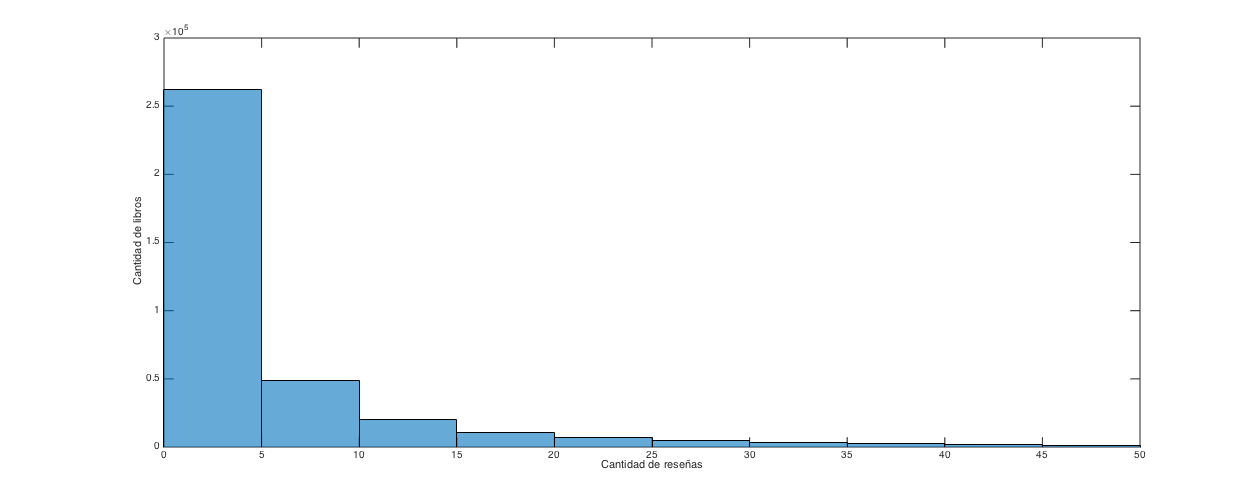
\includegraphics[width=7.5in]{imgs/cantResenasVsCantLibros.png}
  \caption{\small \textit{Cantidad de reseñas por cantidad de libros en dataset crudo}}
  \label{fig:cantResVsCantLibros}
\end{figure} 

El análisis sobre la distribución de la cantidad de reseñas (Figura \ref{fig:cantResVsCantLibros}) muestra que la gran mayoría de los libros presentes en la base de datos posee una cantidad escasa de las mismas. Por ejemplo, el 80\% de los libros tiene menos de 10 reseñas. Por este motivo, decidimos utilizar aquellos libros con 40 o más reseñas para asegurarnos de que el puntaje promedio sea representativo. Esto nos deja con un total de 16.402 libros para analizar.

\begin{figure}[H]
  \centering
  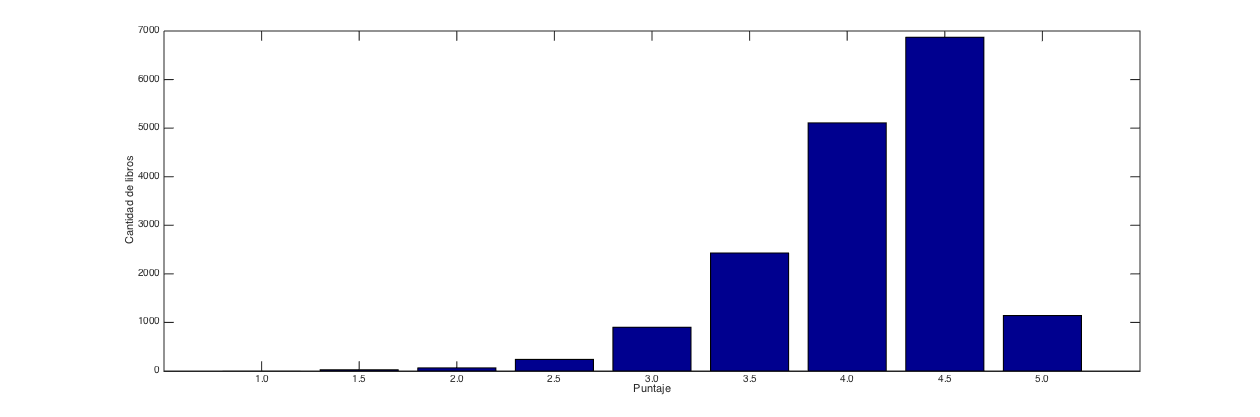
\includegraphics[width=7.5in]{imgs/cantidadDeLibrosVsPuntaje.png}
  \caption{\small \textit{Puntajes por cantidad de libros en dataset refinado}}
  \label{fig:cantLibrosVsPuntaje}
\end{figure} 

El segundo análisis de los libros (Figura \ref{fig:cantLibrosVsPuntaje}) muestra que una amplia porción de éstos se encuentra puntuada entre 4.0 y 4.5, lo que es esperable según algunos estudios\cite{zhang}. Analizando la proporción de los puntajes dentro de agrupaciones de libros por cantidad de reseñas (Figura \ref{fig:cantReseVsCantLibros}), se observa que la misma se mantiene equivalente, lo que evidencia que utilizar libros con 40 o más reseñas es suficiente para asegurar cierta convergencia en los puntajes.

\begin{figure}[H]
  \centering
  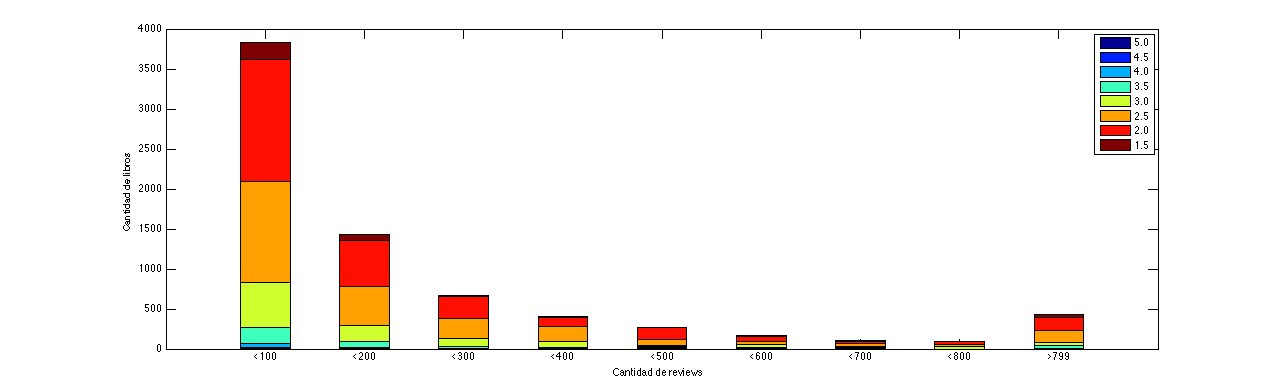
\includegraphics[width=7.5in]{imgs/cantLibrosVScantReviews.png}
  \caption{\small \textit{Cantidad de reseñas por cantidad de libros en dataset refinado}}
  \label{fig:cantReseVsCantLibros}
\end{figure}

\subsection{Análisis de categorías}

En lo que sigue, definimos que existe una relación entre categorías cuando un libro comparte dos de ellas. Al estudiar dichas relaciones, pudimos observar que la cantidad de relaciones es muy grande y que existe una jerarquización de categorías\footnote{http://cor.to/categories} (Figura \ref{fig:jerarquizacionDeCategorias}).

Por otro lado, nos percatamos de que no sólo la mayoría de los libros se encuentra en diversas categorías a la vez sino que estas últimas aparecen acompañadas de todos los subconjuntos de la jerarquía a la que pertenecen. Por ejemplo, la categoría ``Drama'' aparece junto con ``Books'', ``Subjects'' y ``Literature \& Fiction'', por lo que ciertos libros terminan perteneciendo a 16 o más categorías. Para obtener una lista más significativa, eliminamos las que resultaban demasiado generales, demasiado específicas o poco descriptivas como ``Bargain Books'', ``Authors A-Z'', ``Age 3-5'', entre otras. Para esto, confeccionamos una lista de dichas categorías y, para eliminar aquellas demasiado específicas, sacamos las que aparecían 50 veces o menos. Una vez realizada la reducción a 129 categorías, eliminamos manualmente aquellas que nos parecían demasiado generales, obteniendo así una lista final de 113 categorías.

\subsubsection{Homogeneidad de la muestra}

\begin{figure}[H]
  \centering
  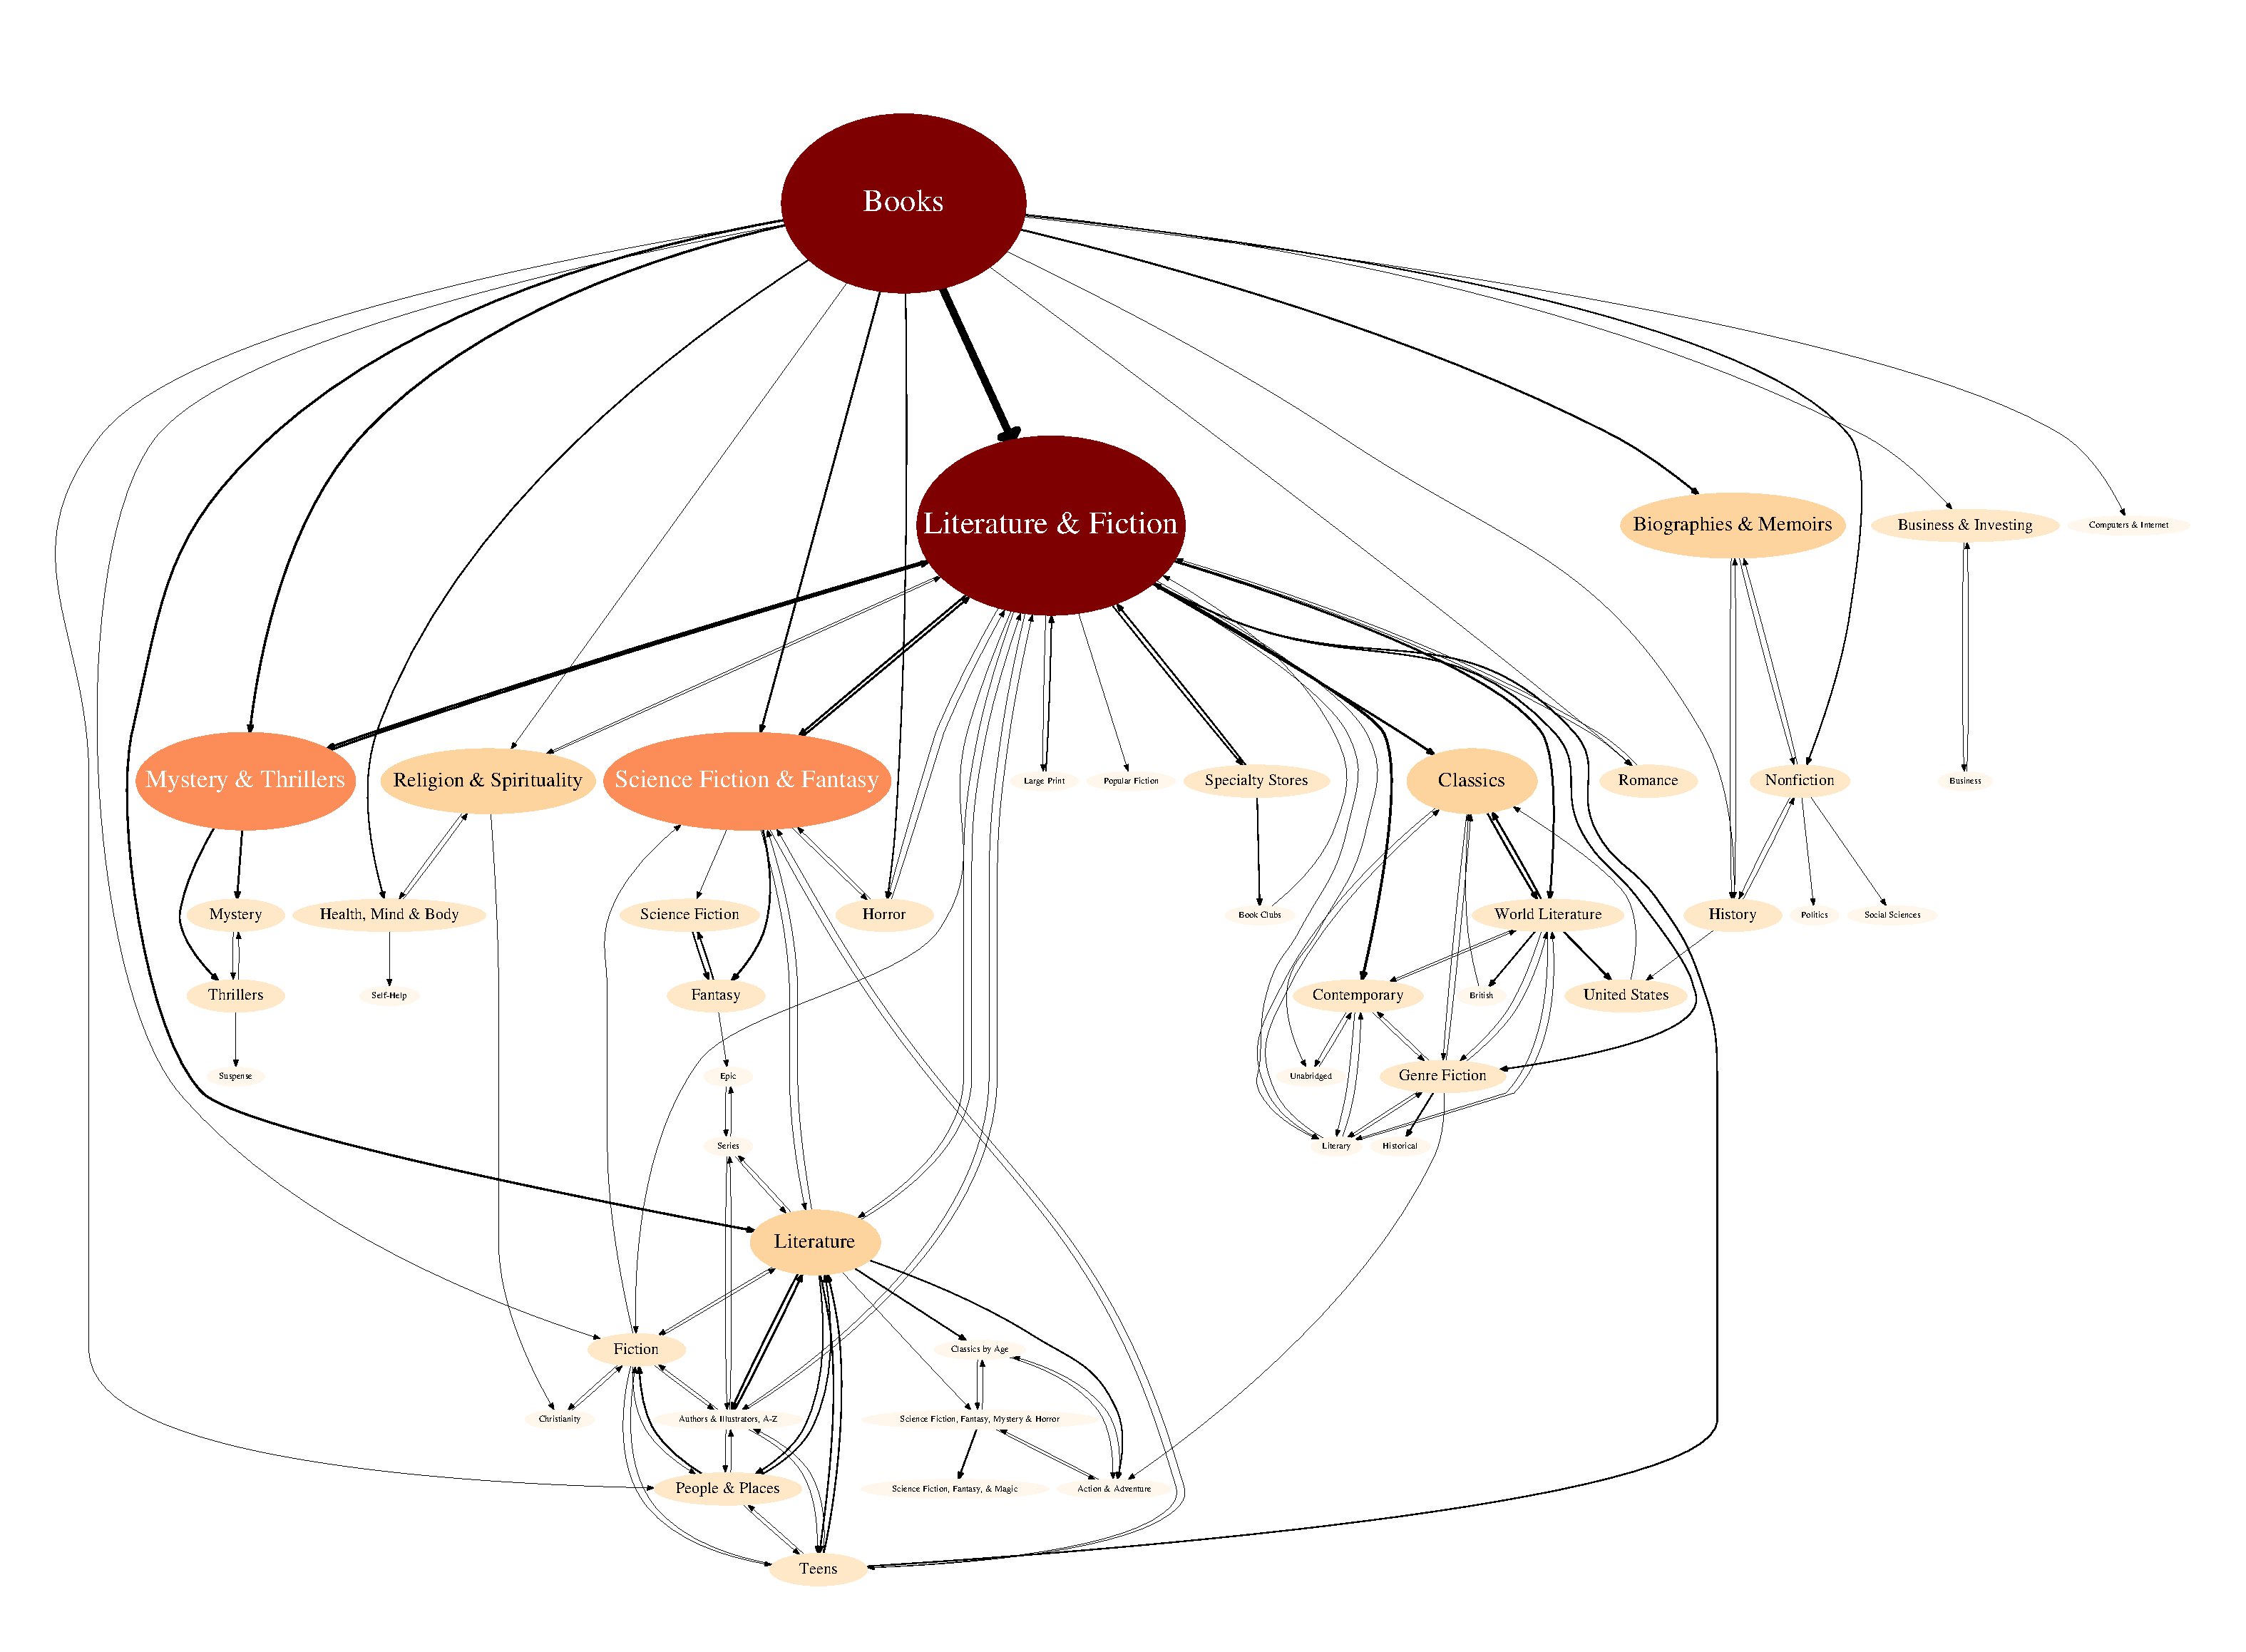
\includegraphics[width=8in]{../results/graph.pdf}
  \caption{\small \textit{Grafo de relaciones entre categorías}}
  \medskip
  \begin{subfigure}{0.90\textwidth}
    \footnotesize La intensidad de los colores y tamaños simbolizan la cantidad de apariciones una categoría, mientras que la intensidad de los trazos la cantidad de apariciones de una relación entre categorías. Definimos que existe una relación entre categorías cuando un libro pertenece a ambas.
  \end{subfigure}
  \label{fig:jerarquizacionDeCategorias}  
\end{figure}

A partir de la lista de categorías, realizamos una codificación de la base de datos en donde cada libro puede ser descripto como una tira de ceros y unos. Cada cero o uno indica la pertenencia o no a una categoría. Utilizando Weka\footnote{http://www.cs.waikato.ac.nz/ml/weka/}, ejecutamos el algoritmo de clusterización \textit{Expectation Maximization} con 10 folds y 8 clusters. 

Si bien nuestro objetivo original era obtener 4 clusters, al especificar dicha cantidad uno de los clusters agrupaba demasiados libros dado que el algoritmo agrupaba todos aquellos que no podía terminar de clasificar (por el límite asignado) en uno solo. Como todos los clusters comparten categorías, la agrupación totalmente disjunta de éstos es imposible. Sin embargo, los formamos minimizando la cantidad de libros que comparten categorías con otros clusters. Probamos distintas maneras de agruparlos y, finalmente, la composición quedó definida de la siguiente manera:\\

\begin{itemize}
\item \textbf{Cluster Nº1:} Science Fiction and Fantasy, Classics, Fantasy, World Literature
\item \textbf{Cluster Nº2:} Religion and Spirituality, Fiction, Health Mind and Body, Self-Help
\item \textbf{Cluster Nº3:} Mystery and Thrillers, Thrillers, Biographies and Memoirs, Suspense, Nonfiction, History, Politics, Social Science
\item \textbf{Cluster Nº4:} Other categories
\end{itemize}

~

De esta manera, sólo el 20\% de los libros comparte categorías de 2 clusters distintos. Un primer análisis de las cantidades contenidas en cada cluster (Cuadro \ref{table:puntajecluster}) muestra que, si bien la división está lejos de ser perfecta en lo que respecta a cantidades nominales, nos da margen suficiente para analizar libros de distintos puntajes y clusters.

~

\begin{table}[H]
 \centering
  \begin{tabular}{| l | l | l | l | l |}
  \hline
  \diagbox[width=10em]{Puntaje}{Cluster} & 1 & 2 & 3 & 4 \\
  \hline
  1.5  & 4     & 2    & 19   & 5    \\
  \hline
  2    & 6     & 4    & 35   & 27   \\
  \hline
  2.5  & 36    & 33   & 103  & 66   \\
  \hline
  3    & 107   & 139  & 414  & 237  \\
  \hline
  3.5  & 450   & 390  & 855  & 733  \\
  \hline
  4    & 1394  & 863  & 1483 & 1366 \\
  \hline
  4.5  & 1801  & 1661 & 1610 & 1800 \\
  \hline
  5    & 232   & 355  & 230  & 322  \\
  \hline
    Total & 4030  & 3447 & 4749 & 4556 \\
    \hline
  \end{tabular}
  \caption{\small \textit{Cantidad de libros de cada cluster dividida en sus respectivas reseñas}}
	\label{table:puntajecluster}
\end{table}


\section{Experimentos y Resultados}\label{sec:expyres}

Para verificar nuestra hipótesis inicial, realizamos un experimento aplicando cada una de las métricas a una selección de libros. Sobre los resultados, analizamos preliminarmente los gráficos obtenidos para luego verificar mediante un test de hipótesis nuestra asunción inicial.

\subsection{Procedimiento experimental}

Por lo que pudimos observar, los puntajes promedios de las reseñas en la base de datos de Amazon toman a lo sumo 10 valores distintos: desde 0 a 5 en intervalos de 0.5. Utilizando los clusters como medio de referencia, seleccionamos alrededor de 15 libros por cada puntaje promedio distinto dentro de cada cluster, totalizando aproximadamente 600 libros. Sin embargo, los libros pertenecientes a los puntajes promedios más bajos (0 a 2.5) fueron difíciles de hallar, por lo que decidimos compactar dicho rango y utilizar 15 libros para el mismo, con un total entonces de 364 libros.

Cada uno de los libros fue convertido de su formato original a texto plano, removiendo cualquier tipo de carácter especial. Luego, se realizó una tokenización (utilizando \textit{tokenizer}\footnote{http://moin.delph-in.net/WeSearch/DocumentParsing}) de cada uno de los textos, para posteriormente aplicar \textit{readability}\footnote{https://pypi.python.org/pypi/readability} y obtener los resultados finales.

\subsection{Análisis preliminar de resultados}

Una vez obtenidos los resultados (Figura \ref{fig:boxplots}), realizamos un análisis preliminar a través de boxplots utilizando percentiles. Como cada una de las métricas devuelve valores en distintas escalas, normalizamos los resultados para poder compararlos fácilmente. En el caso de Flesch-Kincaid, además de normalizar invertimos sus valores para poder evidenciar la misma relación que en el resto de las métricas.


\begin{figure}[H]
\centering
\begin{subfigure}{0.27\textwidth}
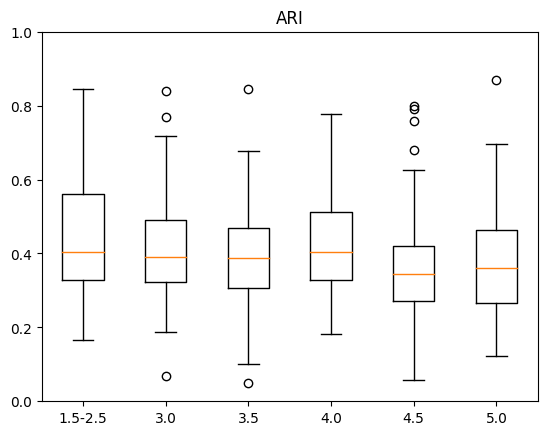
\includegraphics[scale=0.41]{../unigrams/scripts/boxplots/ARI.png}
\end{subfigure} \hspace{0.05\textwidth}
\begin{subfigure}{0.27\textwidth}
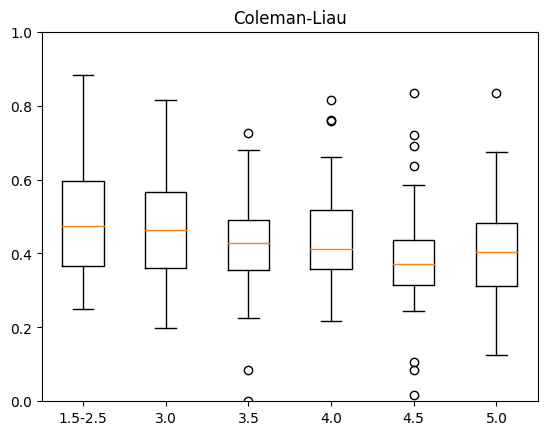
\includegraphics[scale=0.41]{../unigrams/scripts/boxplots/Coleman-Liau.png}
\end{subfigure} \hspace{0.05\textwidth}
\begin{subfigure}{0.27\textwidth}
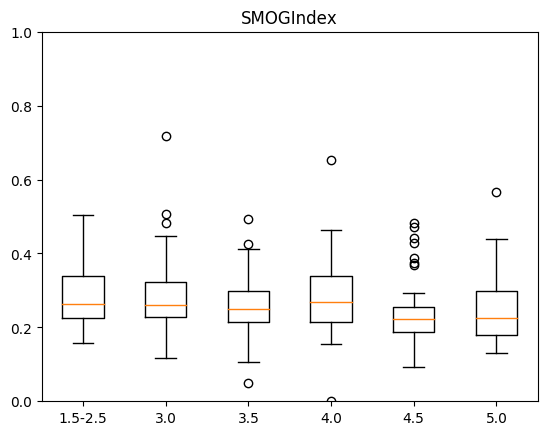
\includegraphics[scale=0.41]{../unigrams/scripts/boxplots/SMOGIndex.png}
\end{subfigure}
\end{figure}

\begin{figure}[H]
\centering
\begin{subfigure}{0.27\textwidth}
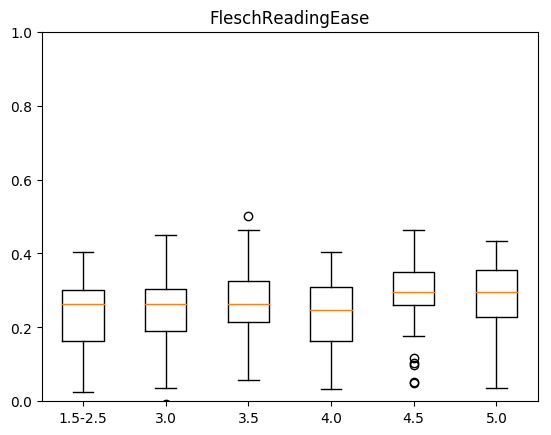
\includegraphics[scale=0.41]{../unigrams/scripts/boxplots/FleschReadingEase.png}
\end{subfigure} \hspace{0.05\textwidth}
\begin{subfigure}{0.27\textwidth}
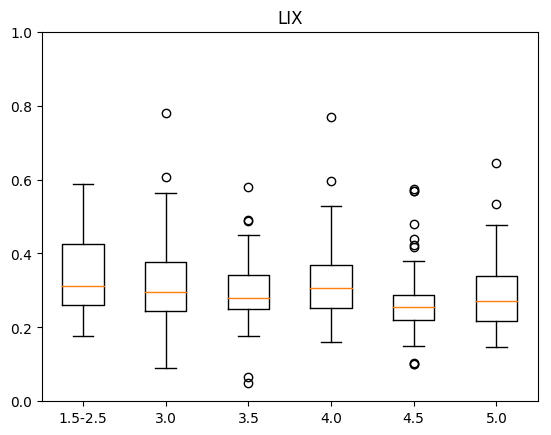
\includegraphics[scale=0.41]{../unigrams/scripts/boxplots/LIX.png}
\end{subfigure} \hspace{0.05\textwidth}
\begin{subfigure}{0.27\textwidth}
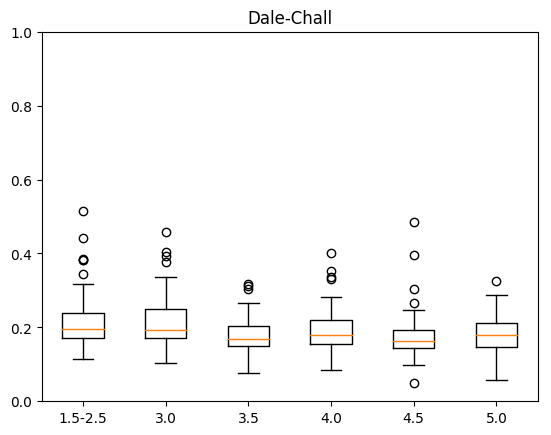
\includegraphics[scale=0.41]{../unigrams/scripts/boxplots/Dale-Chall.png}
\end{subfigure}
\caption{\small \textit{Boxplots sobre los resultados normalizados de cada métrica}}
\medskip
\begin{subfigure}{0.80\textwidth}
\footnotesize Resultados obtenidos de la aplicación de las métricas al conjunto de libros seleccionados. Las medias están simbolizadas en naranja, los limites de las cajas denotan los cuartiles, las líneas muestran el rango de los datos y los círculos denotan outliers.
\end{subfigure}
\label{fig:boxplots}
\end{figure}

En todos los casos, podemos observar una leve tendencia descendente en los valores de las métricas a medida que el puntaje promedio aumenta. Sin embargo, es difícil discernir a simple vista si las diferencias son significativas.

\subsection{Realización y resultados del test de hipótesis}

Para determinar si la diferencia entre dos resultados es significativa, el procedimiento estándar consiste en realizar un test de hipótesis. En nuestro caso, decidimos utilizar el estadístico Kolmogorov-Smirnov de dos vías. El mismo plantea como hipótesis nula que dos muestras independientes se consiguen de la misma distribución continua. Rechazando esta hipótesis, confirmamos que las dos muestras fueron tomadas de distribuciones distintas y, dado que estamos utilizando los resultados de una misma métrica, la diferencia debe provenir de los textos analizados.

Para plantear los tests de hipótesis correspondientes, utilizamos la función $ks\_2samp$\footnote{https://docs.scipy.org/doc/scipy-0.15.1/reference/generated/scipy.stats.ks\_2samp.html} de la librería scipy que computa el estadístico Kolmogorov-Smirnov dadas dos muestras. Luego, dados dos arreglos \textbf{a} y \textbf{b} se obtienen \textbf{D} (o estadístico KS) y el p-valor correspondiente a \textbf{D}. El estadístico consiste en:
$$D_{n}=\sup_{x}|F_{n}(x)-F(x)|$$
siendo $F(x)$ la función de distribución acumulada. Luego, si el estadístico KS es pequeño o el p-valor grande, no podemos rechazar la hipótesis de que las dos muestras son de la misma distribución\cite{degroot}.\\

La hipótesis nula es rechazada con nivel de significación $\alpha$ si:
\begin{equation} \label{eq:1}
D > C(\alpha) = c(\alpha) \cdot \sqrt{\frac{n_1+n_2}{n_1\cdot n_2}}
\end{equation}
donde $n_1$ y $n_2$ son los tamaños de las muestras a comparar y el valor de $c(\alpha)$ se define como:
$$c(\alpha) = \sqrt{1/2\cdot log(\alpha/2)}$$

Para ejecutar el script, seleccionamos como muestras los conjuntos de libros de los 4 clusters con las reseñas $2.5-3.0$ y $4.5-5.0$. De esta forma, nos aseguramos una cantidad de libros adecuada para obtener resultados significativos. Los resultados obtenidos con un nivel de significancia de $\alpha = 0.001$ (o sea $C(0.001) = 0.2506$) para las métricas analizadas fueron los siguientes:\\

\begin{table}[H]
\begin{center}
  \begin{tabular}{ | l | l | l | l | }
  \hline
  Métrica & P-valor & D & ¿Rechaza la hipótesis nula?\\
  \hline
  ARI & 1.9e-2 & 1.929e-2 & \textbf{NO} (1.9e-2 $< \alpha$ y $C(\alpha) <$ 1.929e-2)\\
  \hline
  LIX & 1.684e-3 & 2.378e-1 & \textbf{NO} (1.684e-3 $< \alpha$ y $C(\alpha) <$ 2.378e-1)\\
  \hline
  Coleman-Liau & 5.97e-4 & 2.546e-1 & \textbf{Sí} (5.97e-4 $< \alpha$ y $C(\alpha) <$ 2.546e-1)\\
  \hline
  FleschReadingEase & 9.126e-05 & 2.82e-1 & \textbf{Sí} (9.126e-05 $< \alpha$ y $C(\alpha) <$ 2.82e-1)\\
  \hline
  Dale-Chall & 2.52e-05 & 3e-1 & \textbf{Sí} (2.52e-05 $< \alpha$ y $C(\alpha) <$ 3e-1)\\
  \hline
  SMOGIndex & 8.01e-06 & 3.15e-1 & \textbf{Sí} (8.01e-06 $< \alpha$ y $C(\alpha) <$ 3.15e-1)\\
  \hline
  \end{tabular}
  \caption{\small \textit{Resultados del estadístico Kolmogorov-Smirnov sobre los valores de las métricas}}
  \medskip
  \begin{subfigure}{0.80\textwidth}
    \footnotesize Se compararon los valores obtenidos entre un grupo de libros con puntajes mínimos y otro con puntajes máximos utilizando un test de hipótesis. Pueden observarse en la tabla los p-valores, el estadístico (D) y la condición de rechazo para cada una de las métricas.
  \end{subfigure}
  \label{table:resultadoMetricas}
  \end{center}
  \end{table}

Como se puede observar en el Cuadro \ref{table:resultadoMetricas}, en 4 de 6 métricas la hipótesis nula fue rechazada para un nivel de significancia bajo. Es importante remarcar que las métricas que fallan en rechazar el test de hipótesis son, probablemente, las menos confiables. Además, si se usa un nivel de significancia un poco más alto, como lo es $\alpha = 0.05$ (o sea $C(0.05) = 0.1746$), todas las métricas rechazan la hipótesis nula (datos no mostrados). Otra variable a tener en cuenta es que posiblemente 364 libros no sean suficientes para las métricas con mayor p-valor ya que al aumentar la cantidad de muestras el p-valor disminuye y la condición de aceptación de $D$ (\ref{eq:1}) es más fácilmente satisfacible.

\begin{figure}[H]
\begin{center}
  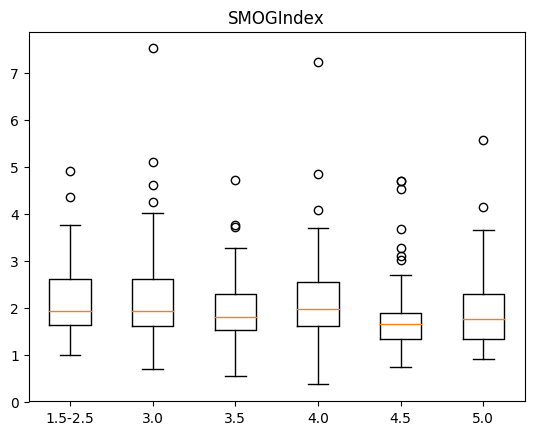
\includegraphics[width=3.5in]{../unigrams/scripts/boxplots/not-normalized-SMOGIndex.png}
  \caption{\small \textit{Boxplot de SMOGIndex}}
  \label{fig:boxplotSMOG}
  \end{center}
\end{figure}

Si analizamos en detalle el boxplot generado en base a los valores devueltos por la métrica SMOG (Figura \ref{fig:boxplotSMOG}), podemos ver que éstos están centrados alrededor del 8, lo que significa que una persona con 8 años de educación debería ser capaz de entender la mayoría de los libros. En el histograma de la Figura \ref{fig:histoSMOG} realizado para analizar la distribución de los valores, podemos ver que la mayoría de los libros se encuentra entre 7 y 9, tendencia que se puede observar también en el resto de las métricas, evidenciando así que una gran parte de los libros utilizados para el análisis no son difíciles de leer. Por lo tanto, es esperable que las diferencias en las medianas entre los dos grupos analizados no sean muy grandes.

\begin{figure}[H]
\begin{center}
  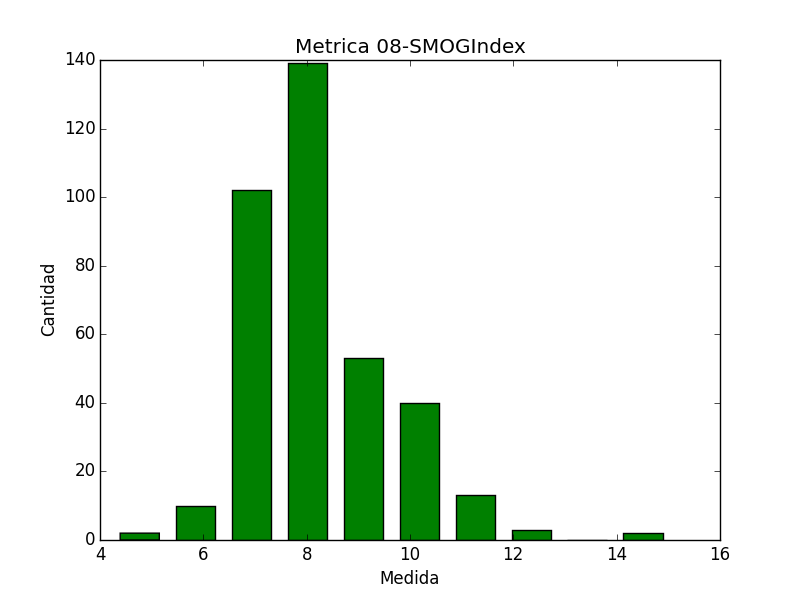
\includegraphics[width=4.0in]{../unigrams/scripts/histogram/08-SMOGIndexhistogram.png}
  \caption{\small \textit{Cantidad de libros por valores de SMOGIndex}}
  \label{fig:histoSMOG}
  \end{center}
\end{figure}

Para dar algunos ejemplos concretos sobre los valores resultantes de aplicar la métrica a libros, seleccionamos los de menor y mayor requerimiento de años y uno cercano a la mediana. El libro ``Day No Pigs Would Die'' de ``Robert Newton Peck'' requiere, según la métrica SMOG, 5 años de educación para ser entendido y tiene un puntaje promedio de 3.5. Según los comentarios que pueden ser leídos en la página de Amazon\footnote{https://www.amazon.com/dp/1883332052} pareciera ser un libro con una historia pobre y escrito de manera burda. Por otro lado, el libro ``A New Kind of Science'' de ``Stephen Wolfram'' requiere 15 años de educación y tiene un puntaje promedio de 3. Éste, según los comentarios\footnote{https://www.amazon.com/dp/1579550088}, trata sobre algunos temas de ciencias de la computación, por lo que tiene sentido que su lenguaje sea más complicado. Sin embargo, es un libro que desagrada a muchos usuarios ya que trata como nuevos a temas que son bien conocidos en el ámbito y se extiende mucho sobre los mismos, probablemente por ignorancia del autor\footnote{https://www.amazon.com/review/R2NIU9I3JQZP5J}. Finalmente, el libro ``Watership Down'' de ``Richard Adams'' requiere 7 años de educación y tiene un puntaje promedio de 4.5. Este libro aparenta ser literatura clásica y posee muy buenas reseñas por parte de los usuarios\footnote{https://www.amazon.com/dp/1565115864}.


\section{Conclusiones y trabajo futuro}\label{sec:conclusion} 

En el presente trabajo, evidenciamos que en líneas generales existe una relación entre el puntaje promedio de las reseñas que le dan los lectores a un libro y su legibilidad. Todas las métricas que utilizamos, en mayor o menor medida y con una acotada cantidad de libros para su análisis, presentaron evidencia de dicha relación. Es posible que con una mayor cantidad de libros y métricas más avanzadas se pueda estudiar más en profundidad el comportamiento de esta última y se pueda llegar a resultados más concretos.

En un trabajo futuro, sería interesante analizar el conjunto de libros con una métrica multi-variable y elementos de procesamiento de lenguaje natural, como lo es \textit{Coh-Metrix}\cite{graesser}. Este tipo de métricas describe mejor la forma en que el libro está escrito y, por lo tanto, podría evidenciar más fácilmente la relación estudiada. Además, sería interesante repetir el análisis con más y actualizada información (ya que el dataset posee 7 años de antigüedad), de forma tal de poder analizar puntualmente cada categoría y observar si existe alguna variación de los resultados de cada una de ellas.

Es importante remarcar que durante la búsqueda de algunos de los libros pudimos observar que en el transcurso de estos 7 años su puntaje aumentó en Amazon. Como nombramos anteriormente, algunos estudios indican que éste es un comportamiento esperado a lo largo del tiempo\cite{zhang}, por lo que si bien llamó nuestra atención, no nos pareció preocupante.

\begin{figure}[H]
\begin{center}
  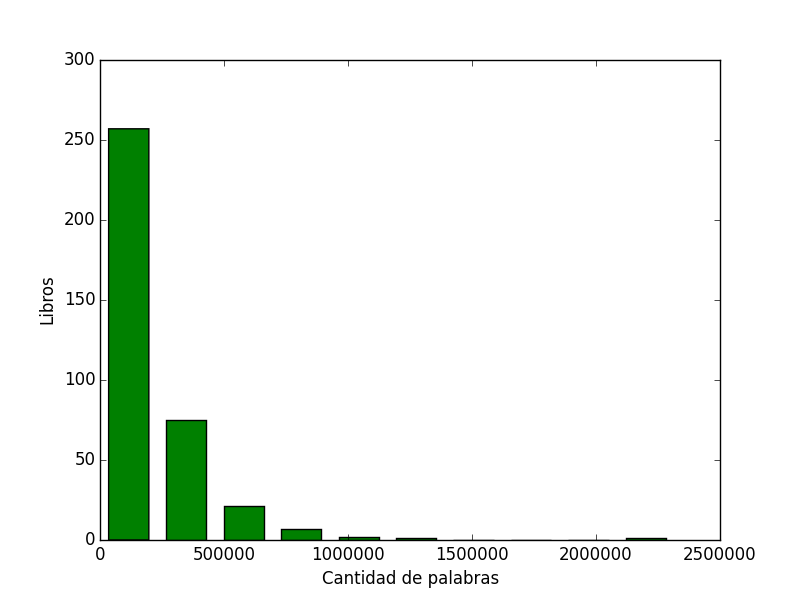
\includegraphics[width=3.5in]{../unigrams/scripts/histogram/histogramaDePalabras.png}
  \caption{\small \textit{Cantidad de palabras por cantidad de libros}}
  \label{fig:cantPalabrasVsCantLibros}
  \end{center}
\end{figure}

Varias de las métricas mencionadas, como ARI y Flesch–Kincaid Reading Ease, hacen uso de la cantidad de palabras en los textos para determinar su legibilidad. Ya que un análisis de la cantidad de palabras en los libros analizados muestra una distribución similar a los puntajes de las reseñas (Figura \ref{fig:cantPalabrasVsCantLibros}), podría ser interesante en un trabajo futuro, analizar la correlación de dicho valor con los resultados de las métricas, analizando si la representación de resultados se comportan de la misma forma.

\begin{thebibliography}{1}

\bibitem{hu} Nan Hu, Paul A Pavlou, and Jennifer Zhang, ``Can online reviews reveal a product’s true quality?: empirical findings and analytical modeling of online wordof-mouth communication,''\hskip 1em plus
  0.5em minus 0.4em\relax in \emph{Proceedings of the 7th ACM conference on Electronic commerce}. ACM, 2006, pp. 324–330.
  
\bibitem{talwar} Arjun Talwar, Radu Jurca, and Boi Faltings, ``Understanding user behavior in online feedback reporting,''\hskip 1em plus
  0.5em minus 0.4em\relax in \emph{Proceedings of the 8th ACM conference on Electronic commerce}. ACM, 2007, pp. 134–142.

\bibitem{muchnik} Lev Muchnik, Sinan Aral, and Sean J Taylor,``Social influence bias: A randomized experiment,''\hskip 1em plus
  0.5em minus 0.4em\relax \emph{Science, vol. 341(6146)}, pp. 647–651, August 2013.

\bibitem{zhang}
Zhang, Yaonan, et al. ``Online ratings: Convergence towards a positive perspective?.'' \hskip 1em plus
  0.5em minus 0.4em\relax \emph{Acoustics, Speech and Signal Processing (ICASSP)}, 2014 IEEE International Conference on. IEEE, 2014.

\bibitem{chevalier}
Judith A Chevalier and Dina Mayzlin, ``The effect of word of mouth on sales: Online book reviews,'' \hskip 1em plus
  0.5em minus 0.4em\relax \emph{Journal of marketing research}, vol. 43, pp. 354–54, August 2006.

\bibitem{fowler}
G. A. Fowler and J.D. Avila, ``On the internet, everyone’s a critic but they’re not very critical,'' \hskip 1em plus
  0.5em minus 0.4em\relax \emph{Wall Street Journal}, 2009.

\bibitem{leskovec}
J. Leskovec, L. Adamic and B. Adamic. ``The Dynamics of Viral Marketing''.\hskip 1em plus
  0.5em minus 0.4em\relax \emph{ACM Transactions on the Web (ACM TWEB)}, 1(1), 2007.

\bibitem{graesser}
Graesser,~A.~C.,~McNamara,~D.~S.,~Louwerse,~M.~M., \& Cai,~Z. (2004). ``Coh-Metrix: Analysis of text on cohesion and language.''\footnote{http://cor.to/graesser} \hskip 1em plus
  0.5em minus 0.4em\relax \emph{Behavior Research Methods,Instruments, \& Computers}, 36(2), 193-202.

\bibitem{crossley}
Crossley,~S.~A.,~Allen,~D.~B., \& McNamara,~D.~S. (2011). ``Text Readability and Intuitive Simplification: A Comparison of Readability Formulas.''\hskip 1em plus
  0.5em minus 0.4em\relax \emph{Reading in a foreign language}, 23(1), 84-101.

\bibitem{diuk}
Diuk,~C.~G.,~Slezak,~D.~F.,~Raskovsky,~I.,~Sigman,~M., \& Cecchi,~G.~A. (2012). ``A quantitative philology of introspection.''\hskip 1em plus
  0.5em minus 0.4em\relax \emph{Frontiers in integrative neuroscience}, 6.
  
\bibitem{orlow} 
Paasche-Orlow MK, Taylor HA, Brancati FL (2003)`` Readability standards for informed-consent forms as compared with actual readability''.\hskip 1em plus
  0.5em minus 0.4em\relax \emph{New England Journal of Medicine} 348: 721–726.
  
\bibitem{klare} 
Klare GR (1974) ``Assessing readability''.\hskip 1em plus
  0.5em minus 0.4em\relax \emph{Reading Research Quarterly} 10: 62–102.
  
\bibitem{kanungo} 
Kanungo T, Orr D (2009) ``Predicting the readability of short web summaries''.\hskip 1em plus
  0.5em minus 0.4em\relax \emph{Proceedings of the Second ACM International Conference on Web Search and Data Mining} (WSDM ’09). New York: ACM Press. 202–211.
  
\bibitem{karmakar} 
Karmakar S, Zhu Y (2010) ``Visualizing multiple text readability indexes''.\hskip 1em plus
  0.5em minus 0.4em\relax \emph{2010 International Conference on Education and Management Technology} (ICEMT). Washington, DC: IEEE. 133–137.

\bibitem{izgi} 
Izgi, Umit, and Burcu Sezginsoy Seker. ``Comparing different readability formulas on the examples of science-technology and social science textbooks.''\hskip 1em plus
  0.5em minus 0.4em\relax \emph{Procedia-Social and Behavioral Sciences} 46 (2012): 178-182.

\bibitem{mcclure}
McClure, Glenda M. ``Readability formulas: Useful or useless?.''\hskip 1em plus
  0.5em minus 0.4em\relax \emph{IEEE Transactions on Professional Communication 1} (1987): 12-15.
  
\bibitem{smog}
Mc Laughlin, G. Harry. ``SMOG grading-a new readability formula.''\hskip 1em plus
  0.5em minus 0.4em\relax \emph{Journal of reading 12.8} (1969): 639-646.

\bibitem{ari-flesch}
Kincaid, J. Peter, et al. ``Derivation of new readability formulas (automated readability index, fog count and flesch reading ease formula) for navy enlisted personnel.''\hskip 1em plus
  0.5em minus 0.4em\relax No. RBR-8-75. \emph{Naval Technical Training Command Millington TN Research Branch}, 1975.

\bibitem{lix-rix}
Anderson, Jonathan. ``Lix and rix: Variations on a little-known readability index.''\hskip 1em plus
  0.5em minus 0.4em\relax \emph{Journal of Reading} 26.6 (1983): 490-496.

\bibitem{coleman-liau}
Coleman, Meri, and Ta Lin Liau. ``A computer readability formula designed for machine scoring.''\hskip 1em plus
  0.5em minus 0.4em\relax \emph{Journal of Applied Psychology} 60.2 (1975): 283.

\bibitem{dale-chall}
Dale, Edgar, and Jeanne S. Chall. ``A formula for predicting readability: Instructions.''\hskip 1em plus
  0.5em minus 0.4em\relax \emph{Educational research bulletin} (1948): 37-54.

\bibitem{dale-chall-ex}
Chall, Jeanne Sternlicht, and Edgar Dale. ``Readability revisited: The new Dale-Chall readability formula.''\hskip 1em plus
  0.5em minus 0.4em\relax \emph{Brookline Books}, 1995.
  
\bibitem{liang} 
Liang, Franklin Mark. Word Hy-phen-a-tion by Com-put-er. \hskip 1em plus
  0.5em minus 0.4em\relax \emph{Department of Computer Science, Stanford University}, 1983.
  
\bibitem{hedman}
Hedman, Amy S. ``Using the SMOG formula to revise a health-related document.'' \hskip 1em plus
  0.5em minus 0.4em\relax \emph{American Journal of Health Education} 39.1 (2008): 61-64.
  
\bibitem{degroot} DeGroot, Morris H., and Mark J. Schervish. ``Probability and statistics, Fourth Edition''. \hskip 1em plus
  0.5em minus 0.4em\relax \emph{Addison-Wesley}, 2012. P663-665

\end{thebibliography}

\end{document}


